% Free range VHDL
% Authors: Bryan Mealy, Fabrizio Tappero
% Date: May, 2011
%
% (C) 2011 B. Mealy, F. Tappero
%
% !TEX root = master.tex
%
\chapter{Appendix A: VHDL Reserved Words}
Table \ref{vhdl_ref_words} provides a complete list of VHDL reserved words.

\begin{table}[!h]
\centering
\small\textsf{
\begin{tabular*}{0.9\textwidth}{@{\extracolsep{\fill}} l l l l l }
\hline
abs            &  downto    &  library  &  postponed  &  srl        \\
\rowcolor{light-gray} access         &  else      &  linkage  &  procedure  &  subtype    \\
after          &  elsif     &  literal  &  process   &  then        \\
\rowcolor{light-gray} alias          &  end       &  loop     &  pure      &  to          \\
all            &  entity    &  map      &  range     &  transport   \\
\rowcolor{light-gray} and            &  exit      &  mod      &  record    &  type        \\
architecture   &  file      &  nand     &  register  &  unaffected  \\
\rowcolor{light-gray} array          &  for       &  new      &  reject    &  units       \\
assert         &  function  &  next     &  rem       &  until       \\
\rowcolor{light-gray} attribute      &  generate  &  nor      &  report    &  use         \\
begin          &  generic   &  not      &  return    &  variable    \\
\rowcolor{light-gray} block          &  group     &  null     &  rol       &  wait        \\
body           &  guarded   &  of       &  ror       &  when        \\
\rowcolor{light-gray} buffer         &  if        &  on       &  select    &  while       \\
bus            &  impure    &  open     &  severity  &  with        \\
\rowcolor{light-gray} case           &  in        &  or       &  signal    &  xnor        \\
component      &  inertial  &  others   &  shared    &  xor         \\
\rowcolor{light-gray} configuration  &  inout     &  out      &  sla       &              \\
constant       &  is        &  package  &  sll       &              \\
\rowcolor{light-gray} disconnect     &  label     &  port     &  sra       &              \\
\hline
\end{tabular*}}
\caption{A complete list of VHDL reserved words.}
\label{vhdl_ref_words}
\end{table}

% blank page
\null\newpage
\thispagestyle{empty}
\mbox{}

\chapter{Appendix B: Standard VHDL Packages}
After years of development by the US Department of Defense, in February 1986 all VHDL rights were transferred to the Institute of Electrical and Electronics Engineers (IEEE) which since then has carried on the process of standardisation of the language. 

After three main language standardisation steps that took place in 1987, 1993 and in 2002, VHDL now includes a large set of packages that, once included in your code, give to the user the possibility of using several mathematical constants, numerical functions, overloaded operators, type conversion functions, enhanced signal types and much more.

The main VHDL language library packages that you will probably need to use in your career as an engineer can be included in your code by using the following statements:

\begin{verbatim}
library IEEE;
use IEEE.std_logic_1164.all;
use IEEE.std_logic_arith.all;
use IEEE.numeric_bit.all;
use IEEE.numeric_std.all;
use IEEE.std_logic_signed.all;
use IEEE.std_logic_unsigned.all;
use IEEE.math_real.all;
use IEEE.math_complex.all;
\end{verbatim}

For instance, the inclusion of the package \texttt{std\_logic\_1164} in your code, will give you the ability of using the assignment operator \texttt{=} between two different data types. The following listing shows a simple coding example of some of the many advantages of using these libraries.
\newpage
\clearpage

\begin{lstlisting}[caption=Example of operators and types available with some IEEE packages.]
-- typical packages declaration
library IEEE;
use ieee.std_logic_1164.all ;
use ieee.std_logic_arith.all ;
use ieee.std_logic_unsigned.all ;

-- entity
entity my_blk is 
    port (  IN1, IN2  : in  std_logic; 
            CLK,OUT1  : in  std_logic); 
end my_blk;

-- architecture
architecture arch of my_blk is
signal A, B : std_logic_vector(7 downto 0) ;
signal Y    : std_logic_vector(8 downto 0) ;
signal X    : integer range 0 to 255 ;
begin
   sync_proc: process(CLK,CLR)
   begin
     if CLR = '1' then 
        OUT1 <= '0';  
     elsif rising_edge(CLK) then -- std_logic_1164 gives "rising_edge()"
        Y <= A + B + IN1;        -- std_logic_arith overloads the addition operator
        X <= CONV_INTEGER(A);    -- std_logic_arith gives "CONV_INTEGER()"
        OUT1 <= IN1 AND IN2; 
     end if; 
   end process sync_proc; 
end arch;
\end{lstlisting}
As it comes clear from the previous listing, the inclusion of these three main standard libraries allows you to write very powerful VHDL code. A quite useful cheat-sheet about VHDL standard libraries and what they can offer is available from here:
\begin{verbatim}
http://www.vhdl.org/rassp/vhdl/guidelines/vhdlqrc.pdf
http://www.vhdl.org/rassp/vhdl/guidelines/1164qrc.pdf
\end{verbatim}

The IEEE standardized libraries heavily enhance the VHDL language capability giving you a long list of functions that you can freely use in your VHDL source code. A list of these libraries cannot be included here for obvious copyright reasons but all IEEE libraries source code is freely available to you from the following link:

\url{http://standards.ieee.org/downloads/1076/1076.2-1996/}

Alternatively, the same VHDL libraries can be browsed and downloaded from the GHDL website:

\url{http://ghdl.free.fr}

Finally, the software developing tool (e.g. Xilinx ISE) that you use for the synthesis of your VHDL code will include these libraries. A quick look at the source code will give you a pretty good idea of what is available to you and how to use it. For instance, a quick look at the \texttt{math\_real.vhdl} library, available from: 

\url{http://standards.ieee.org} 

will shows you that the constant of type real \texttt{MATH\_PI = 3.1415926} is soon available to you as soon as you include the \texttt{"use IEEE.math\_real.all;"} line. The square root function \texttt{SQRT()} is just another example.

\chapter{Appendix C: VHDL Reference Cards}
Here-below you can find two sets of very useful VHDL reference cards made by Qualis Design Corporation.

\begin{verbatim}
http://www.vhdl.org/rassp/vhdl/guidelines/vhdlqrc.pdf
http://www.vhdl.org/rassp/vhdl/guidelines/1164qrc.pdf
\end{verbatim}

\newpage\clearpage
\thispagestyle{empty}
\begin{textblock*}{174mm}(1mm,0mm)
%\textblockcolour{red}
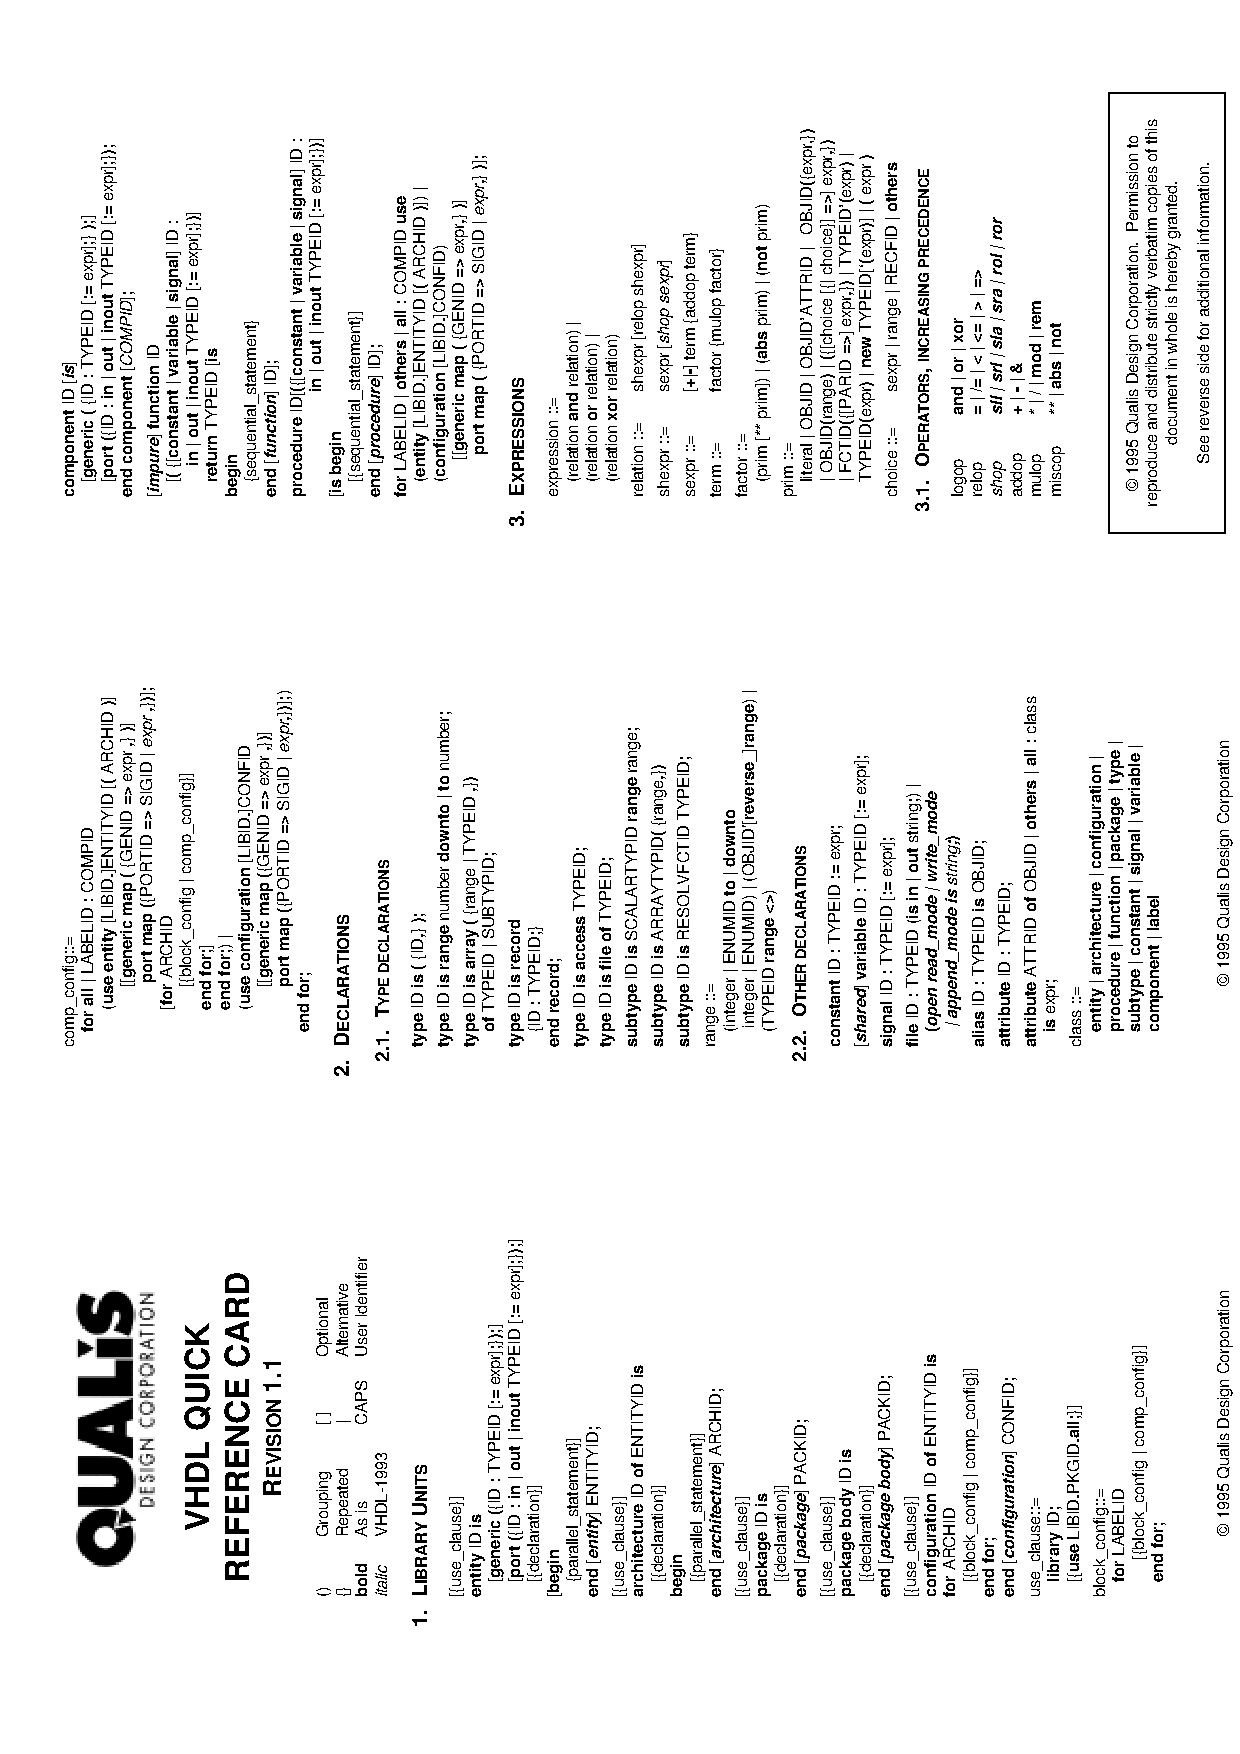
\includegraphics[width=169mm]{ref_cards/qr1.pdf}
\end{textblock*}
\null\newpage

\thispagestyle{empty}
\begin{textblock*}{174mm}(1mm,0mm)
%\textblockcolour{red}
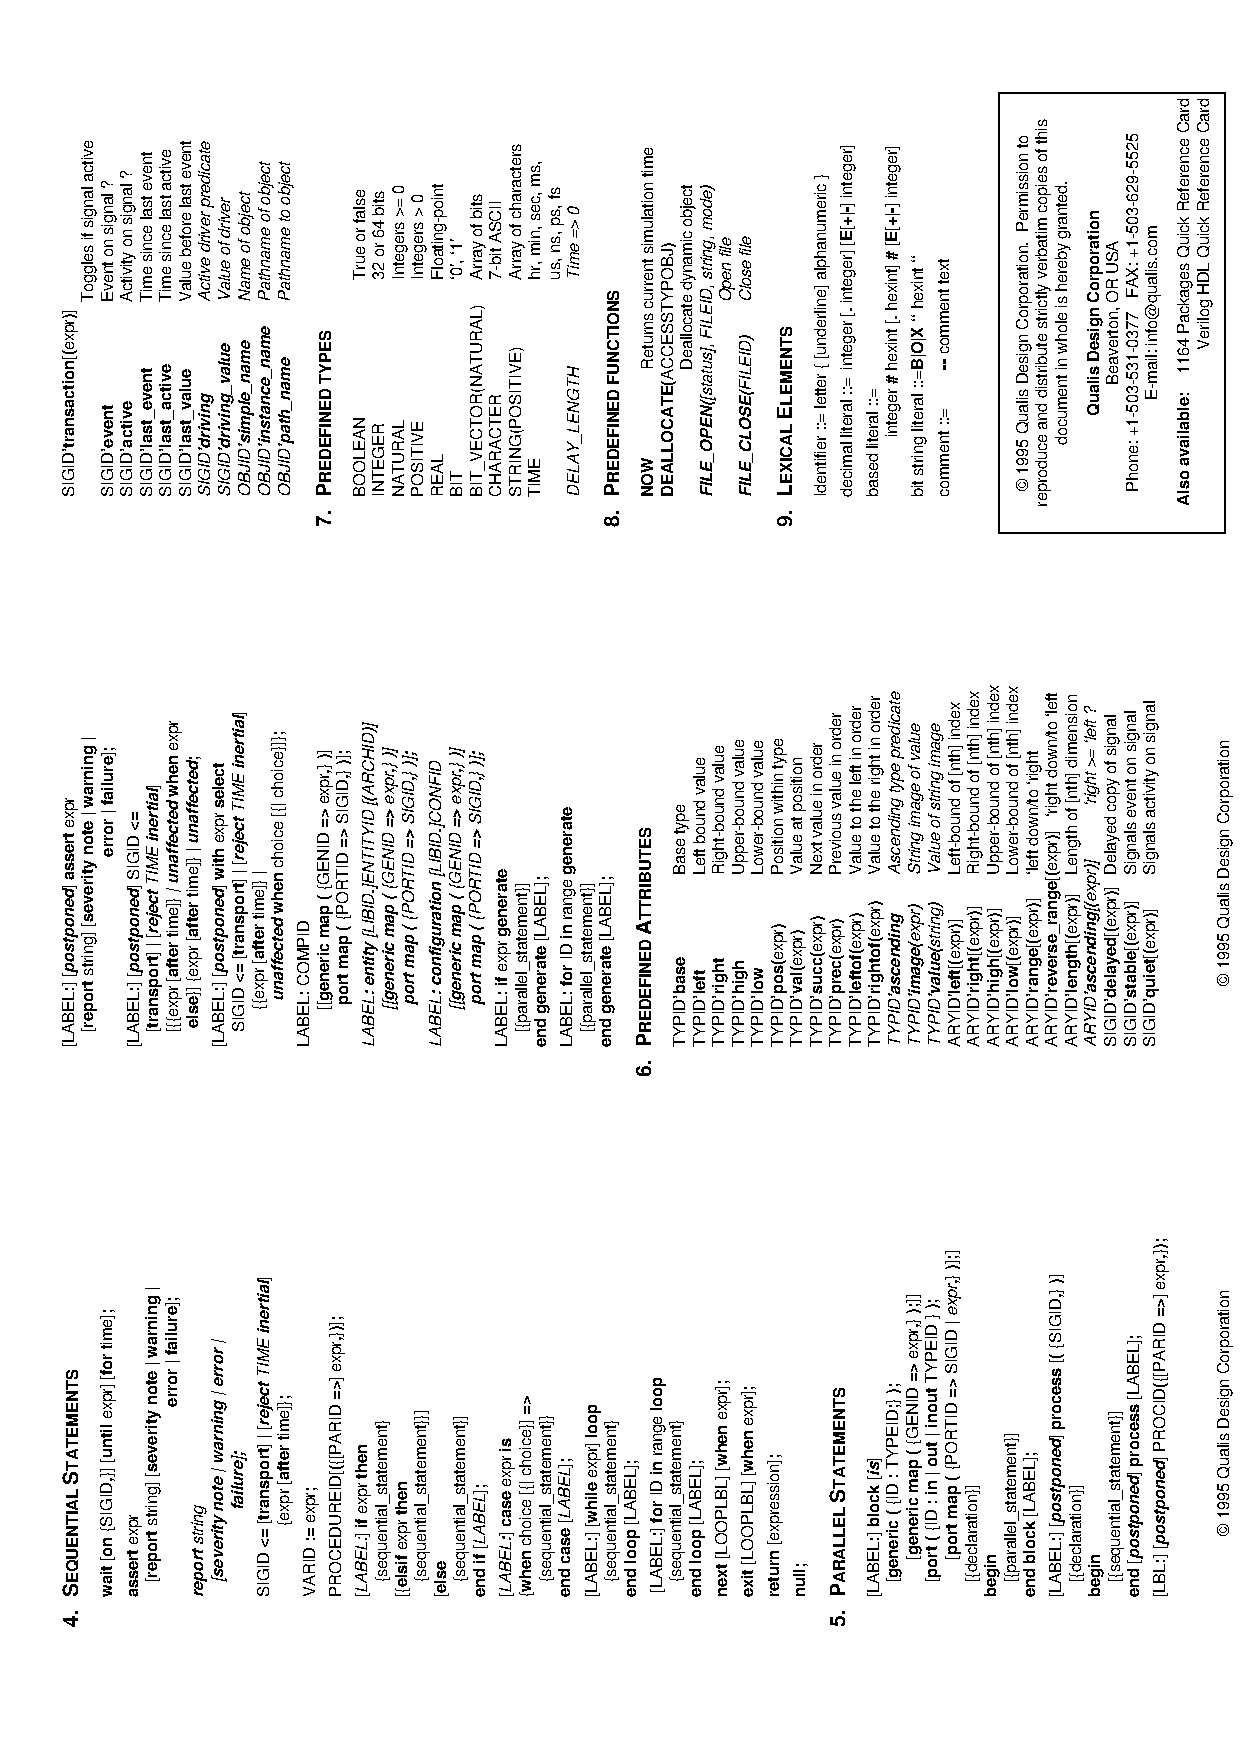
\includegraphics[width=169mm]{ref_cards/qr2.pdf}
\end{textblock*}
\null\newpage

\thispagestyle{empty}
\begin{textblock*}{174mm}(1mm,0mm)
%\textblockcolour{red}
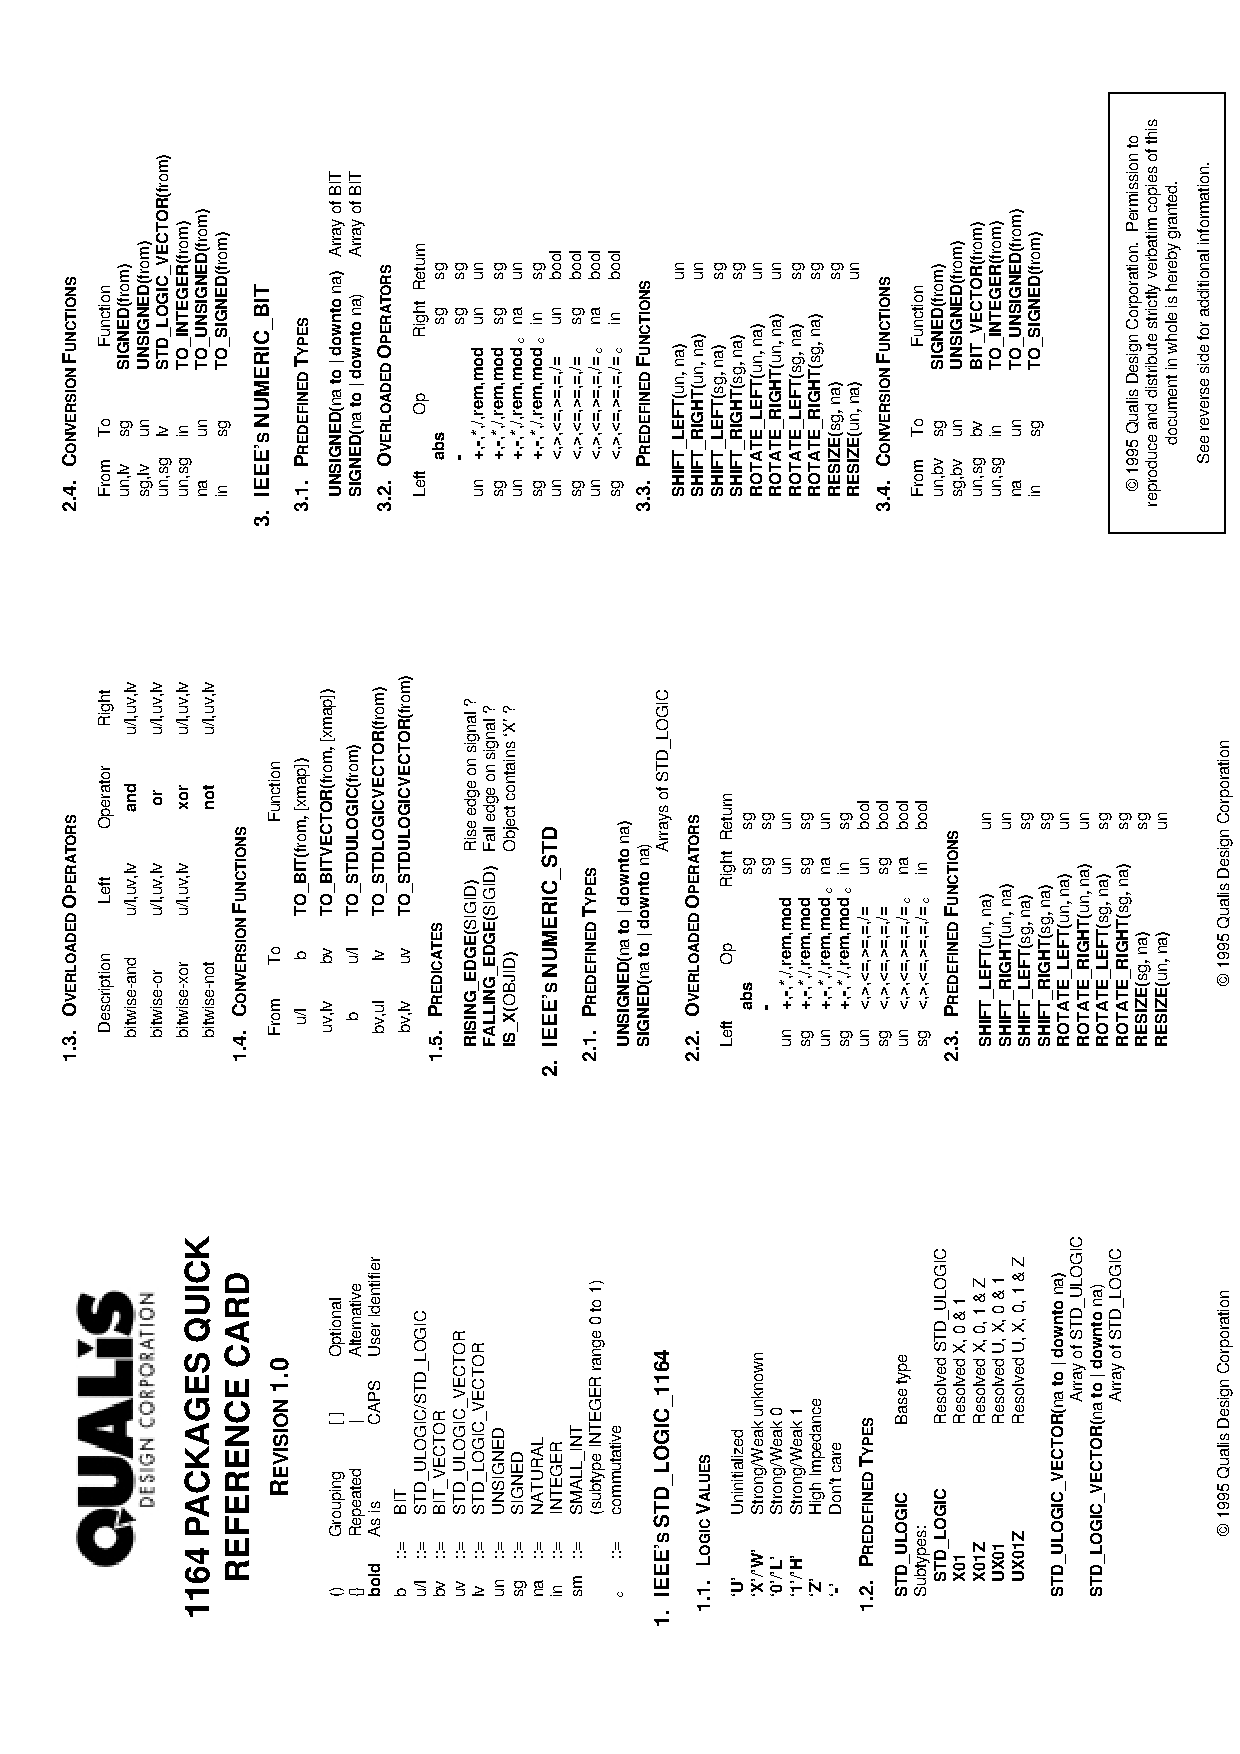
\includegraphics[width=169mm]{ref_cards/qr3.pdf}
\end{textblock*}
\null\newpage

\thispagestyle{empty}
\begin{textblock*}{174mm}(1mm,0mm)
%\textblockcolour{red}
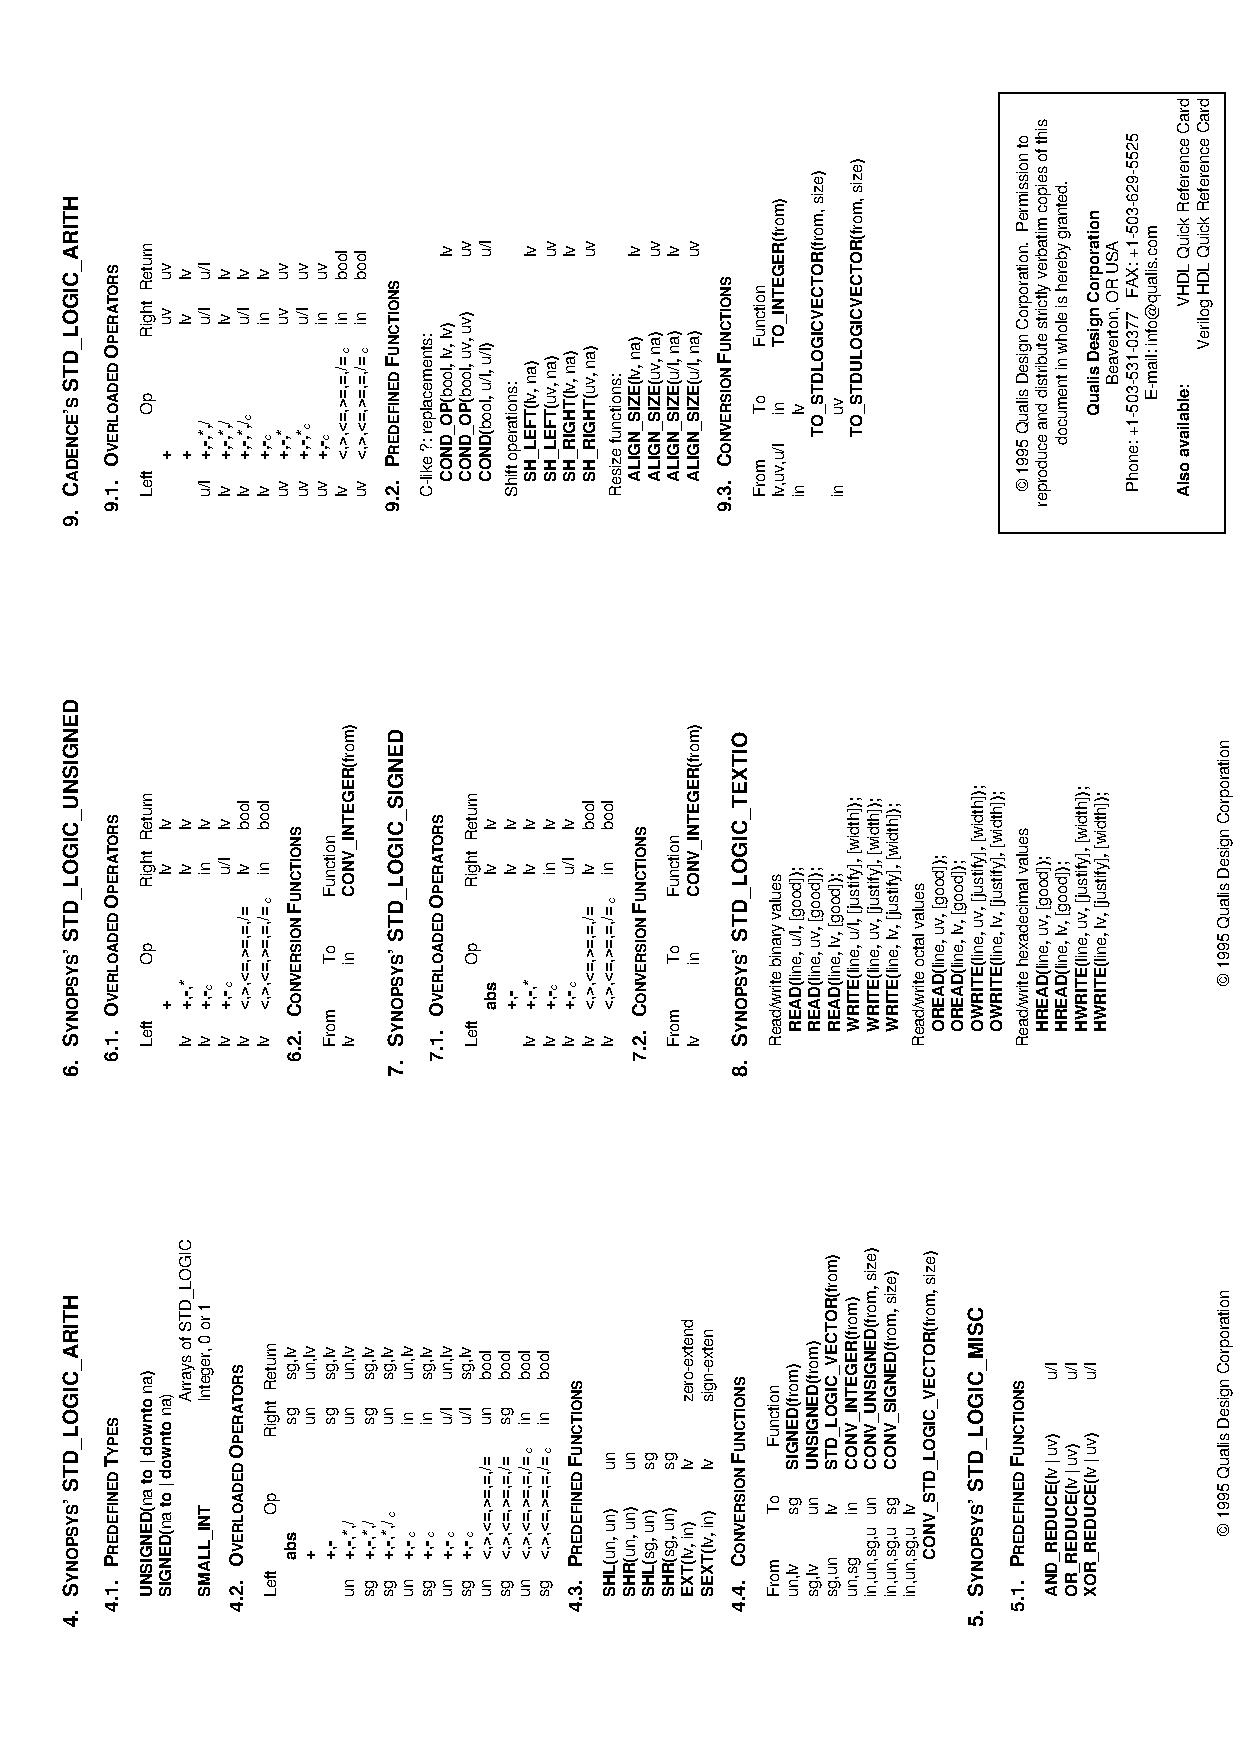
\includegraphics[width=169mm]{ref_cards/qr4.pdf}
\end{textblock*}
\null\newpage

